
\section{Pre-training} 
\label{app:pt}


\subsection{Model architectures and training regimes}
\label{app:pt-model-arch}

We pretrain models from different families (\llama{} and \olmo{}), of different sizes (up to 4B), and under different training regimes (20 TPP and 140 TPP), yielding the following five model setups: \llamazeropointfiveB{}, \llamaoneB{}, \llamafourB{}, \olmoonex{}, \olmosevenx{}. Model details are in Table~\ref{table:model-arch}. For each model setup, we pretrain variants with varying weight decay values.


\renewcommand{\arraystretch}{1.2} 
\begin{table}[H]
\centering
\begin{tabular}{llllll}
\hline
\textbf{} & \textbf{Llama-2-0.5B} & \textbf{Llama-2-1B} & \textbf{Llama-2-4B} & \textbf{OLMo-2-1B}  \\ \hline
Model size        & 0.5B     & 1B      & 4B       & 1.5B       \\
Hidden size       & 1536     & 2048    & 4096     & 2048      \\
Intermediate size & 3216     & 4896    & 7792     & 16384      \\
Vocab size        & 32000    & 32000   & 32000    & 100278    \\
Context length    & 2048     & 2048    & 2048     & 4096      \\
\# Heads          & 32       & 32      & 32       & 16        \\
\# Layers         & 20       & 22      & 28       & 16        \\
\# Query groups   & 4        & 4       & 4        & 16         \\ \hline
\end{tabular}
\vspace{0.2cm}
\caption{\textbf{Model architectures.} We use \llama{} model architectures from \citet{qi2025evolm} and \olmo{} model architecture from \citet{olmo2024olmo2}. \llama{} models are trained at 20 TPP and \olmo{} models are trained at 20 TPP and 140 TPP.}
\label{table:model-arch}
\end{table}


\subsection{Training details}
\label{app:pt-training-details}

The training data size (measured in tokens) for each model is determined by the TPP ratio.

\renewcommand{\arraystretch}{1.2} 
\begin{table}[H]
\centering
\begin{tabular}{llll}
\hline
\textbf{Model} & \textbf{Model Size} & \textbf{TPP Ratio} & \textbf{Training Data Size} \\ \hline
\llamazeropointfiveB{} & 0.5B & 20 & 10 BT              \\
\llamaoneB{} & 1B & 20 & 20 BT              \\
\llamafourB{} & 4B & 20 & 80 BT              \\
\olmoonex{} & 1.5B & 20 & 30 BT              \\
\olmosevenx{} & 1.5B & 140 & 210 BT             \\ \hline
\end{tabular}
\vspace{0.2cm}
\caption{\textbf{Model configurations and training data sizes.}}
\label{table:training-data-size}
\end{table}


To pre-train \llama{} models, we use up to 8 A100 GPUs or 16 H100 GPUs. To pre-train \olmo{} models, we use 8xH100 GPUs. The OLMo-2-1B-20x models are each trained for 2 days on a single H100 node. The OLMo-2-1B-140x models are trained for 2 weeks on a single H100 node. For all models, we use the AdamW optimizer and standard warmup-cosine learning rate schedule. The only exception is the OLMo-2-1B-140x models, which follow a warmup-stable-decay schedule \cite{hagele2024scaling}. Llama-2 models are pretrained using the repository from \citet{qi2025evolm}. OLMo-2-1B models are pretrained using the  \href{http://github.com/allenai/OLMo}{official repository} from AllenAI. 

For each model, we train variants with various weight decay values specified in Table~\ref{table:wd}. Additional training hyperparameters are in Tables~\ref{table:pt-hyperparams-llama} and \ref{table:pt-hyperparams-olmo}. 

\renewcommand{\arraystretch}{1.2} 
\begin{table}[H]
\centering
\begin{tabular}{ll}
\hline
\textbf{Model} & \textbf{Weight Decay} \\ \hline
\llamazeropointfiveB{} & 10 values: \{0, 0.0001, 0.001, 0.01, 0.1, 0.5, 1.0, 1.5, 3.0, 10.0\} \\
\llamaoneB{}           & 10 values: \{0, 0.0001, 0.001, 0.01, 0.1, 0.5, 1.0, 1.5, 3.0, 10.0\}  \\
\llamafourB{}          & 3 values: \{0, 0.1, 1.0\}              \\
\olmoonex{}            & 11 values: \{0, 0.1, 0.2, 0.3, 0.4, 0.5, 0.6, 0.7, 0.8, 0.9, 1.0\}               \\
\olmosevenx{}          & 4 values: \{0, 0.1, 0.3, 1.0\}                \\ \hline
\end{tabular}
\vspace{0.2cm}
\caption{\textbf{Weight decay values for each model.} We use the \llamafourB{} weight decay 0.1 model from \citet{qi2025evolm} and the \olmosevenx{} weight decay 0.1 model from \citet{bordt2025train}. We pretrain all other models.}
\label{table:wd}
\end{table}



\begin{table}[H]
\centering
\begin{tabular}{llll}
\hline
\textbf{Hyperparameter } & \textbf{\llamazeropointfiveB{}} & \textbf{\llamaoneB{}} & \textbf{\llamafourB{}}  \\ \hline
precision           & bf16-mixed & bf16-mixed & bf16-mixed  \\
global\_batch\_size & 512     & 512     & 1024        \\
max\_seq\_length    & 2048    & 2048    & 2048        \\
lr\_warmup\_ratio   & 0.1     & 0.1     & 0.1          \\
max\_norm           & 1       & 1       & 1            \\
lr                  & 0.00025  & 0.0002  & 0.00015   \\
min\_lr             & 0.000025 & 0.00002 & 0.000015  \\
weight\_decay       & varies   & varies  & varies    \\
beta1               & 0.9      & 0.9     & 0.9         \\
beta2               & 0.95     & 0.95    & 0.95       \\
epoch               & 1        & 1       & 1             \\ \hline
\end{tabular}
\vspace{0.2cm}
\caption{\textbf{Hyperparameters for Llama-2 model pretraining.} For \llama{} models, hyperparameter values follow those in \citet{qi2025evolm}, except for weight decay, which is varied as the independent variable in our experiments.}
\label{table:pt-hyperparams-llama}
\end{table}



\begin{table}[H]
\centering
\begin{tabular}{lll}
\hline
\textbf{Hyperparameter} & \textbf{\olmoonex{}} & \textbf{\olmosevenx{}} \\ \hline
precision           & bf16-mixed & bf16-mixed \\
global\_batch\_size & 512     & 512     \\
max\_seq\_length    & 4096    & 4096    \\
lr\_warmup\_ratio   & 0.1     & 0.1     \\
max\_norm           & 1       & 1       \\
lr                  & 0.0004  & 0.0004  \\
min\_lr             & 0.00004 & 0 \\
weight\_decay       & varies  & varies  \\
beta1               & 0.9     & 0.9     \\
beta2               & 0.95    & 0.95    \\
epoch               & 1       & 1       \\ \hline
\end{tabular}
\vspace{0.2cm}
\caption{\textbf{Hyperparameters for OLMo-2 model pretraining.} For \olmo{} models, hyperparameter values follow the OLMo-2 defaults \citep{olmo2024olmo2}, except for weight decay, which is varied as the independent variable in our experiments.}
\label{table:pt-hyperparams-olmo}
\end{table}



\begin{figure*}[h]
    \centering
    \begin{subfigure}[b]{0.30\textwidth}
        \centering
        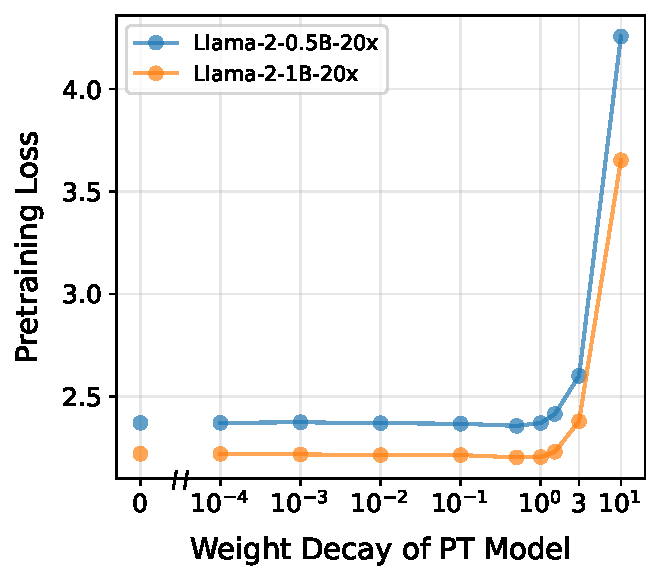
\includegraphics[width=\linewidth]{figs/a04_val_loss/all_models_wd_vs_loss_llamax2_withwd0.pdf}
        \caption{\llama{}-\{0.5B, 1B\}-20x}
    \end{subfigure}
    \hfill
    \begin{subfigure}[b]{0.34\textwidth}
        \centering
        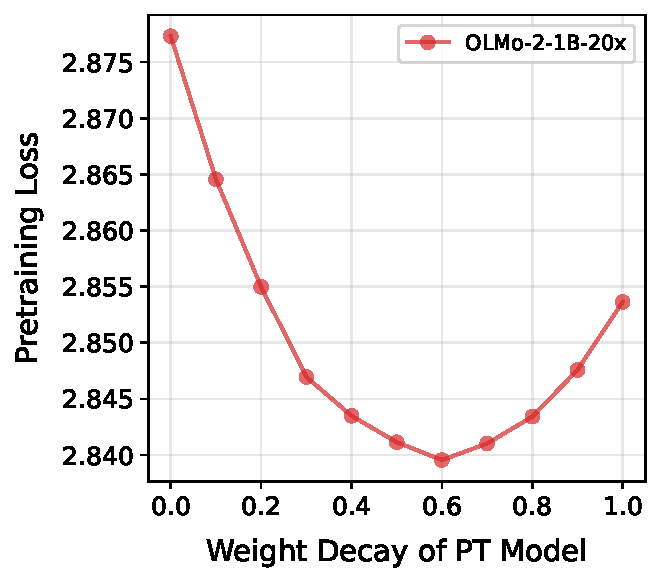
\includegraphics[width=0.88\linewidth]{figs/a04_val_loss/all_models_wd_vs_loss_zoomedin_OLMo-2-1B-20x_withwd0.pdf}
        \caption{\olmoonex{}}
    \end{subfigure}
    \hfill
    \begin{subfigure}[b]{0.34\textwidth}
        \centering
        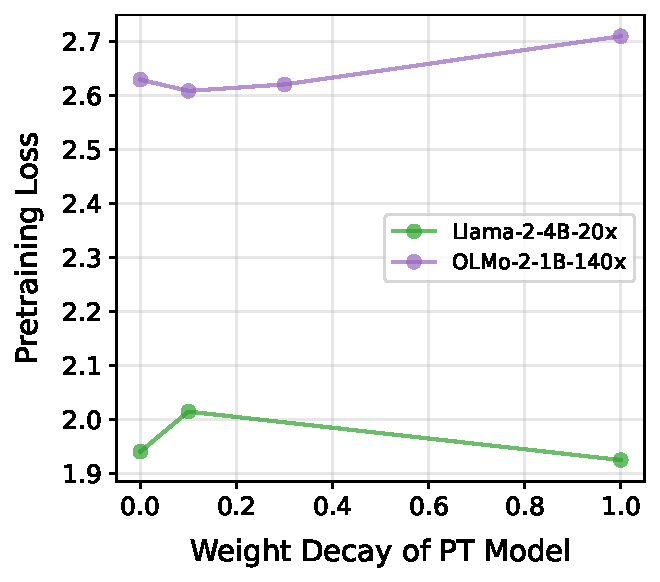
\includegraphics[width=0.88\linewidth]{figs/a04_val_loss/all_models_wd_vs_loss_zoomedin_Llama-2-4B-20x___OLMo-2-1B-140x_withwd0.pdf}
        \caption{\llamafourB{} and \olmosevenx{}}
    \end{subfigure}$\,$\\[4pt]
    \caption{{\bf Pretraining validation cross-entropy loss of models pretrained with varying weight decay.} The weight decay value that minimizes pretraining loss may be equal to or larger than the standard default value of 0.1 depending on the training regime.}
\label{app:fig:pt-val-losses}
\end{figure*}



